\documentclass[]{report}

\usepackage[
	backend = biber,
	style=numeric,
	autocite=plain,
	sorting=none,
	natbib=true
	]{biblatex}
	
\addbibresource{tic-tac-toe-benchmark.bib}

\usepackage{pgfplots}
\pgfplotsset{width=10cm,compat=1.9}
% \usepgfplotslibrary{external} 
% \tikzexternalize 

% Title Page
\title{Tic-Tac-Toe Benchmarks}
\author{Raffaello Bertini}

\begin{document}
\maketitle

\begin{abstract}
	In this report are compared and evaluated all the different implementations of the Minimax algorithm and its variants.
\end{abstract}

\chapter{Intro}

The implementation of the different algorithms \autocite{MIT} has been done with a mixture of imperative, object oriented and functional programming to benchmark also these different code styles.\\

All the algorithms, \textit{Minimax} \autocite{wiki-minimax}, \textit{Negamax} \autocite{wiki-negamax} and \textit{Alpha Beta} \autocite{wiki-alphabeta} with \textit{Transposition Table} \autocite{wiki-transtable}, are implemented in a naive approach, imperative, and then refined to use \textit{traits} and a more functional approach.\\

\paragraph{Minimax}
has been implemented as:
\begin{itemize}
	\item Raw: imperative.
	\item Trait raw: using  OOD.
	\item Trait: OOD combined with functional elements. 
\end{itemize}

\paragraph{Negamax} has been implemented as:
\begin{itemize}
	\item Raw
	\item Trait
\end{itemize}

\paragraph{Alpha Beta} has been implemented as:
\begin{itemize}
	\item Raw
	\item Trait
	\item Raw with transposition table (TT)
\end{itemize}

\paragraph{Transposition Table} has been implemented as:
\begin{itemize}
	\item simple Hash Table
	\item Trait
\end{itemize}

Alpha Beta and Transposition Table are combined to spot differences in the implementation performances.

\chapter{Results}

In this chapter are displayed all the results computed with a Intel I7 CPU.

\section{Tic Tac Toe}
In this section are reported the specific result with the \textit{tic-tac-toe} optimized board game rules.

\begin{table}[]
	\begin{tabular}{|l|lllll}
		\hline
		\multicolumn{1}{|c|}{\textbf{Algorithm}}                                                 & \multicolumn{1}{c|}{\textbf{Time (ms)}} & \multicolumn{1}{c|}{\textbf{Total Calls}} & \multicolumn{1}{c|}{\textbf{cache}} & \multicolumn{1}{c|}{\textbf{cache hits}} \\ \hline
		\multicolumn{1}{|c|}{Minimax Raw}                                                        & \multicolumn{1}{c}{650}                 & \multicolumn{1}{c}{294778}                & \multicolumn{1}{c}{N/A}             & \multicolumn{1}{c}{N/A}                  \\ \cline{1-1}
		\multicolumn{1}{|c|}{\begin{tabular}[c]{@{}c@{}}Minimax \\ Trait\end{tabular}}           & \multicolumn{1}{c}{655}                 & \multicolumn{1}{c}{294778}                & \multicolumn{1}{c}{N/A}             & \multicolumn{1}{c}{N/A}                  \\ \cline{1-1}
		\multicolumn{1}{|c|}{\begin{tabular}[c]{@{}c@{}}Minimax\\ Trait Raw\end{tabular}}        & \multicolumn{1}{c}{808}                 & \multicolumn{1}{c}{294778}	               & \multicolumn{1}{c}{N/A}             & \multicolumn{1}{c}{N/A}                  \\ \cline{1-1}
		\multicolumn{1}{|c|}{\begin{tabular}[c]{@{}l@{}}Negamax\end{tabular}}                    & \multicolumn{1}{c}{308}                 & \multicolumn{1}{c}{294778}                & \multicolumn{1}{c}{N/A}             & \multicolumn{1}{c}{N/A}                  \\ \cline{1-1}
		\multicolumn{1}{|c|}{\begin{tabular}[c]{@{}l@{}}Negamax\\ Trait\end{tabular}}            & \multicolumn{1}{c}{596}                 & \multicolumn{1}{c}{294778}                & \multicolumn{1}{c}{N/A}             & \multicolumn{1}{c}{N/A}                  \\ \cline{1-1}
		\multicolumn{1}{|c|}{\begin{tabular}[c]{@{}l@{}}Alpha Beta\end{tabular}}                 & \multicolumn{1}{c}{75}                  & \multicolumn{1}{c}{12413}                 & \multicolumn{1}{c}{N/A}             & \multicolumn{1}{c}{N/A}                  \\ \cline{1-1}
		\multicolumn{1}{|c|}{\begin{tabular}[c]{@{}l@{}}Alpha Beta\\ Trait\end{tabular}}         & \multicolumn{1}{c}{91}                  & \multicolumn{1}{c}{12413}                 & \multicolumn{1}{c}{N/A}             & \multicolumn{1}{c}{N/A}                  \\ \cline{1-1}
		\multicolumn{1}{|c|}{\begin{tabular}[c]{@{}l@{}}Alpha Beta\\ with TTOld\end{tabular}}    & \multicolumn{1}{c}{260}                 & \multicolumn{1}{c}{4520}                  & \multicolumn{1}{c}{5478}            & \multicolumn{1}{c}{10690}                \\ \cline{1-1}
		\multicolumn{1}{|c|}{\begin{tabular}[c]{@{}l@{}}Alpha Beta\\ with TT\end{tabular}}       & \multicolumn{1}{c}{211}                 & \multicolumn{1}{c}{4520}                  & \multicolumn{1}{c}{5478}            & \multicolumn{1}{c}{10690}                \\ \cline{1-1}
		\multicolumn{1}{|c|}{\begin{tabular}[c]{@{}l@{}}Alpha Beta\\ with TT Trait\end{tabular}} & \multicolumn{1}{c}{137}                 & \multicolumn{1}{c}{4187}                  & \multicolumn{1}{c}{1308}            & \multicolumn{1}{c}{3851}                 \\ \cline{1-1}
	\end{tabular}
	\caption{Tic Tac Toe Solver Results}
	\label{my-label}
\end{table}

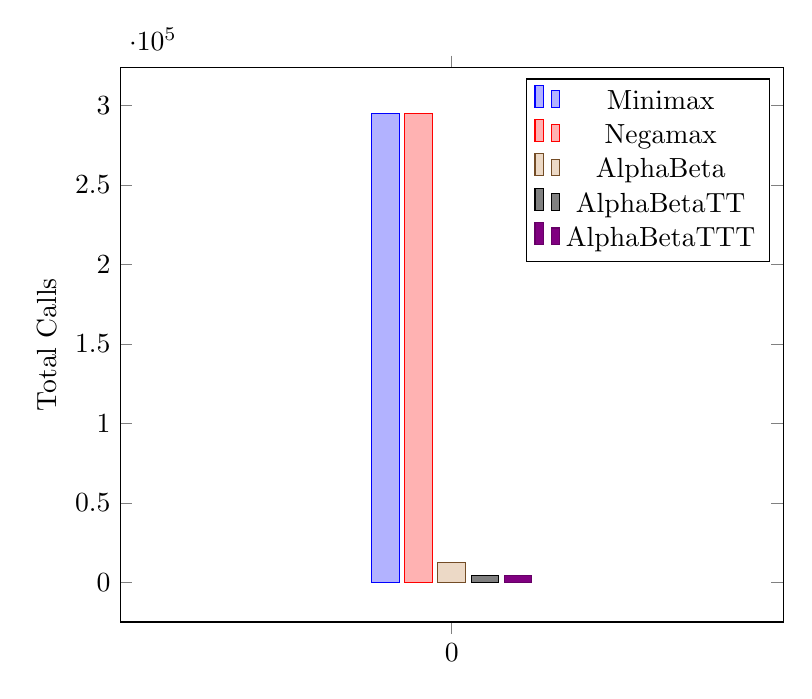
\begin{tikzpicture}
	\begin{axis}[
		x tick label style={/pgf/number format/1000 sep=},
		ylabel={Total Calls},
		ybar,
		xtick=data,
	]
		\addplot coordinates {(0, 294778)};
		\addplot coordinates {(0, 294778)};
		\addplot coordinates {(0, 12413)};
		\addplot coordinates {(0, 4520)};
		\addplot coordinates {(0, 4187)};

		\legend{Minimax, Negamax, AlphaBeta,AlphaBetaTT, AlphaBetaTTT}
	\end{axis}
\end{tikzpicture}

\section{Board 3x3x3}
In this section are reported the specific results with the \textit{board 3x3x3} that are derived from a general \textit{board MxNxK} game rules.
%

\printbibliography

\end{document}          
